\section{Classification pipeline}
Data on the Internet is sometimes questionable. We can use classification to assess the credibility of information found on the web.

\begin{figure}[!ht]
  \centering
  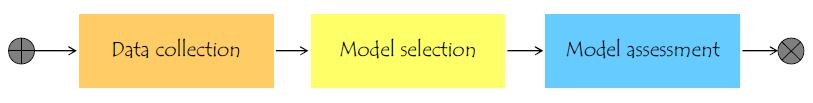
\includegraphics[width=1.0\linewidth]{figures/classification_pipeline}
  \caption{Classification pipeline}
  \label{fig:classificationPipeline}
\end{figure}

\subsection*{Data collection}
Definition of the attributes that describe a data item and the class label. Domain knowledge is needed to know which attributes are relevant for the classification task.

As shown on Figure \ref{fig:dataCollection}, here a the different step in our data collection pipeline:
\begin{enumerate}
	\item Definition of the features that describe a data item
	\item Label the data items to create a training set
	\item Discretisation of the features
	\item Selection of the relevant features
	\item Normalisation of the features
\end{enumerate}

\begin{figure}[!ht]
  \centering
  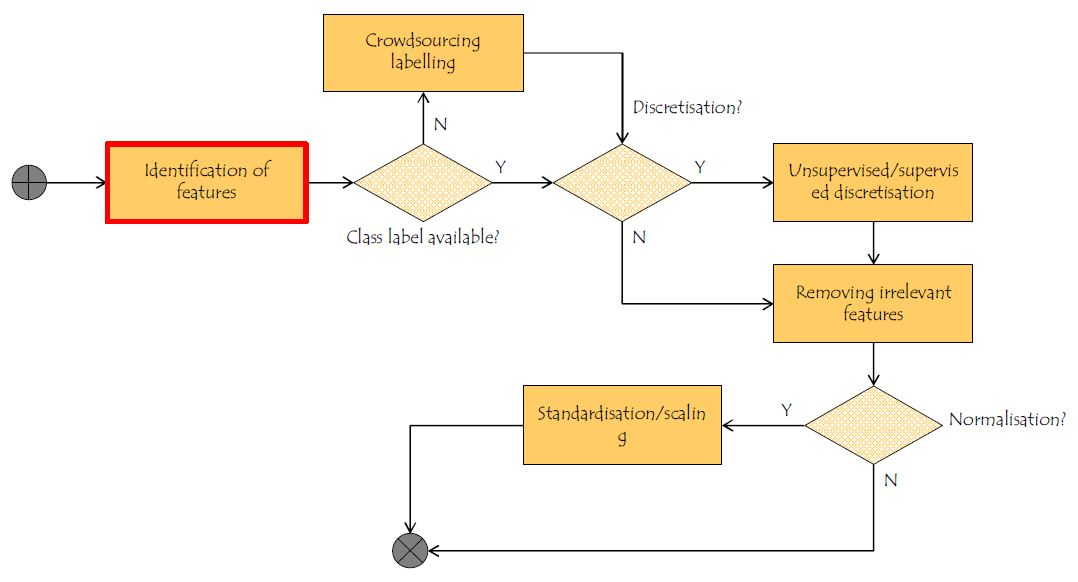
\includegraphics[width=1.0\linewidth]{figures/data_collection}
  \caption{Data collection pipeline}
  \label{fig:dataCollection}
\end{figure}

There exist different types of features:
\begin{itemize}
	\item Numerical (e.g., age, temperature)
	\item Ordinal (e.g., phone code, ...)
	\item Categorical (e.g., student, animals, ...)
\end{itemize}

It is easy to collect data on the web but difficult to label them. The basic idea of crowdsourcing is to enroll a large group of people that will contribute to a specific task. It suits really well for labelling a large data set. However, some of the workers aren't truthful, reliable, and are even sometimes random.

\subsubsection*{Aggregation algorithms}
Given the labelling provided by workers, requester might face the problem of aggregating the answers when they don't coincide.

There are two main classes of aggregation algorithms:
\begin{itemize}
	\item \textbf{Non-iterative}: take the matrix of answers provided by the workers, pre-process it and produce an estimate of the probability that a webpage X is labelled by label L.

	\textbf{Majority decision} algorithm is fast and appropriate for on-line aggregations but very sensitive to spammers. It estimates $P(x_j = l)$ as 
	\begin{align*}
		P(x_j = l) = \frac{1}{N} \sum_{i = 1}^N (1 | a_i(x_j) = j)
	\end{align*}
	with $x_j$ the webpage, $N$ the number of workers, $l$ le label and $a_i(x_j)$ the answer of worker $i$.

	\textbf{Honey pot} algorithm inserts webpages for which the labels are known and will remove workers that fail at correctly labelling more than $m$ of these webpages. It is more robust to spammers but trapping labels are not always available and good workers might be misidentified as spammers if trapping questions are too difficult.

	\item \textbf{Iterative}: take the matrix of answers provided by the worker and produce an estimate of the probability that a webpage X is labelled by label L. With this estimate they update the \textbf{expertise of each worker}, that is, a metric that indicates how good is the worker at performing the labelling task. With this new information, the probability that a webpage X is labelled by label L is estimated again. This cycle continues until convergence.

	\textbf{Expectation Maximisation (EM)} algorithm iterate so as to reduce the expertise of spammers and to increase the expertise of good workers.
	\begin{itemize}
		\item \textbf{E step}: estimate $P(x_j = l)$ as
		\begin{align*}
			P(x_j = l) = \frac{1}{\sum_{i = 1}^N w_i} \sum_{i = 1}^N (w_i | a_i(x_j) = l)
		\end{align*}
		with $w_i$ the expertise weight of worker i

		\item \textbf{M step}: update the expertise $w_i$ as
		\begin{align*}
			w_i = \frac{1}{M} \sum_{j = 1}^M (1 | a_i(x_j) = \argmax_l P(x_j = l))
		\end{align*}
		with $M$ the number of webpages to label
	\end{itemize}

	The EM algorithm is very accurate and very robust to spammers, but slow to converge.
\end{itemize}

\subsubsection*{Discretisation}
\textbf{Unsupervised} discretisation do not take class information into account.
\begin{itemize}
	\item \textbf{Equal width}: divide the range into a predefined number of bins.\\
	$\rightarrow$ lose information is observations are not distributed evenly.
	\item \textbf{Equal frequency}: divide the range into a predefined number of bins so that every interval contains the same number of values.
	$\rightarrow$ many occurences of the same value could be assigned to different bins
	\item \textbf{Clustering}: Perfect for discretisation and can be performed on all the features at the same time.
\end{itemize}

\textbf{Supervised} discretisation take class information into account, measuring the dependency of a discrete interval of values w.r.t the class label. Test that two adjacent intervals of a feature are independent of the class. If they are, merge them.
\textbf{TODO}

\subsubsection*{Feature selection}
\textbf{Filtering}: rank features according to their predictive power and select the best ones.
\begin{itemize}
	\item \textbf{Pros}: independent of the classifier
	\item \textbf{Cons}: assume features are independent
\end{itemize}


Correlation coefficient:
\begin{align*}
	r = \frac{\sum_{i = 1}^n (X_i - \bar{X})(Y_i - \bar{Y})}{\sqrt{\sum_{i = 1}^n (X_i - \bar{X})^2} \sqrt{\sum_{i = 1}^n (Y_i - \bar{Y})^2}}
\end{align*}

Mutual information measures the information that $X$ and $Y$ share:
\begin{align*}
	I(F, C) &= H(C) - H(C | F) = H(F) + H(C) - H(F, C)\\
	H(F) &= - \sum_i P(f_i) \log_2 P(f_i)\\
	H(F, C) &= - \sum_i \sum_j P(f_i, c_j) \log_2 P(f_i, c_j)
\end{align*}
If $I(X, Y) = 0$, knowing X does not tell anything about Y.

The chi-square test checks the independence of the class and the feature, without indicatin the strength or irection of any existing relationship.

\textbf{COULD BE MORE CLEAR}

\textbf{Important}: Collectively relevant features may look individually irrelevant.

\textbf{Wrapper}: starts with no features and add the feature that provide the highest improvement in classification accuracy.
\begin{itemize}
	\item \textbf{Pros}: interact with the classifier and no independence assumption
	\item \textbf{Cons}: computationally intensive
\end{itemize}

\subsubsection*{Feature normalisation}
Some classfiers do not manage well features with very different scales.

\textbf{Standardisation}
\[
	x_i' = \frac{(x_i - \mu_i)}{\sigma_i}
\]
with $\mu_i$ the mean value of feature $x_i$ and $\sigma_i$ its standard deviation.
The drawback of this method is that it assumes that data has been generated by a Gaussian process, which is not always true.

\textbf{Scaling}
\[
	x_i' = \frac{x_i - m_i}{M_i - m_i}
\]
with $M_i$ and $m_i$ the max and min values of feature $x_i$ respectively
The drawback of this method is that it doesn't work well with outliers. The "normal" values will be scale to a very small interval.

\subsection{Model selection}
Once the dataset is ready, we have to select the model that provides the best classification accuracy. 

\begin{figure}[!ht]
  \centering
  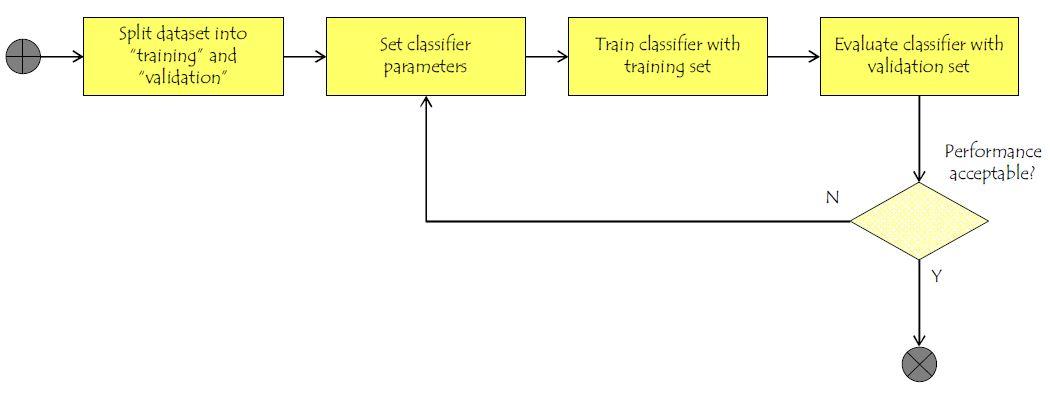
\includegraphics[width=1.0\linewidth]{figures/model_selection}
  \caption{Model selection pipeline}
  \label{fig:modelSelection}
\end{figure}

The task consists in exploring the configuration space of the model in order to find the parameterisation that minimises the loss function.

\begin{itemize}
 	\item \textbf{0-1 loss function} (categorical values)
 	$$ J = \sum_{i = 1}^n \#(y \neq f(x_i)) $$
 	\item \textbf{Squared error} (real values)
 	$$ J = \frac{1}{n} \sum_{i = 1}^n (y_i - f(x_i))^2 $$
 	\item \textbf{Absolute error} (real values)
 	$$ J = \frac{1}{n} \sum_{i = 1}^n |y_i - f(x_i)| $$
 \end{itemize} 

\subsubsection*{Performance metric for Binary Classification}
For categorical binary classification, the usual metrics consider four types of errors as shown on Fig. \ref{fig:binClass}.\\

\begin{figure}[!ht]
  \centering
  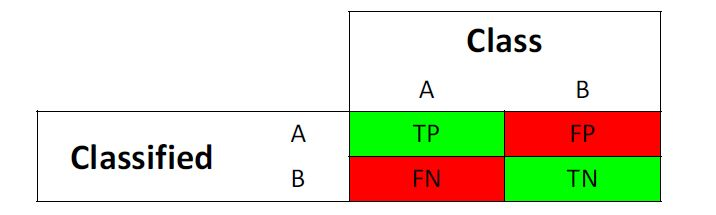
\includegraphics[width=1.0\linewidth]{figures/binary_class}
  \caption{Error types in binary classification}
  \label{fig:binClass}
\end{figure}

\textbf{Accuracy}: the total correct examples divided by the total examples to be classified
$$ A = \frac{TP + TN}{TP + TN + FP + FN} = \frac{TP + TN}{N}$$

\textbf{Precision}: high precision means a few irrelevant examples treates as important
$$ P = \frac{TP}{TP + FP} $$

\textbf{Recall}: high recal means being good at getting the positive class right, fraction of relevant examples that are retrieved.
$$ R = \frac{TP}{TP + FN} $$

\textbf{F-score}: it's necessary to have a unique metrix to compare classifiers.
$$ F1 = 2 \cdot \frac{P \cdot R}{P + R} $$
It is the harmonic mean of precision and recall.

The simplest way to do model selection is constructing a train and validation set. The drawback of this approach is that it does not use all the data to train, and it is possible that the test set is not representative of the classification tasks.

\textbf{Leave-one-out cross validation}
\begin{itemize}
	\item almost unbiased estimate of the true accuracy
	\item time consuming since number of iterations equal number of examples
\end{itemize}

\textbf{K-fold cross validation}: good compromise between having an unbiased estimate and computation time.

\textbf{Bias} and \textbf{variance} can be asessed by comparing the error metrix on the training set and the test set. In the ideal case, we want low bias (small training error) and low variance (small test error). We can observe several cases:
\begin{itemize}
	\item High bias and high variance: worst case
	\item High variance: overfitting $\rightarrow$ should reduce the complexity of the model and add regularisation parameter.
	\item High bias: underfitting $\rightarrow$ should increase complexity of the model and reduce regularisation parameter.
\end{itemize}

\subsection{Model assessment}
Model assessment is the foal of estimating hte classigication oaccuracy of a fixed model.